\chapter{Autonomous Energy Production for Isolated Site (CORRECTION)}


\section*{Prelim}

\begin{enumerate}
    \item $\begin{aligned}
E_{\text{year }}=\overbrace{300 \times 24 \times 365}^{\text{average }}+\overbrace{1500 \times 3 \times 0.5 \times 365}^{\text{peak}} &=  3.45 \text{ MWh/year}\\
&=  9.45 \text{ kWh/day} 
\end{aligned}$

\item $\text{With } 1520 \text{ kWh} / \text{m}^2 / \text{year}$

\vspace{0.25cm}
$\begin{aligned}
& \left.\begin{array}{l}
\eta_{\text{PV}}=20 \% \\
\eta_{\text{Elec}}=90 \%
\end{array}\right\} 18 \% \Rightarrow 270 \text{ kWh} / \mathrm{m}^2 / \text{year (Elec energy)}
\end{aligned}$

\[S=\frac{3.45 \cdot 10^3}{270}=12.8 \text{m}^2\]

\item Number of panels: $\frac{12.8}{1,13 \times 1,06}=10,7 \Rightarrow 11$ panels.\ ($1.13 = $ Surface of 1 panel)

\end{enumerate}

\section{Boost Converter}

\begin{figure}[h]
    \centering
    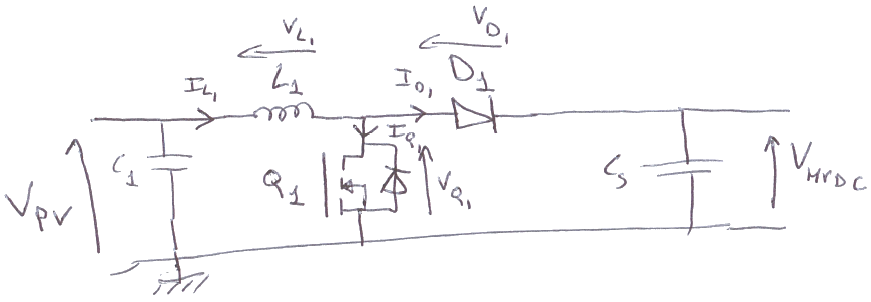
\includegraphics[width=\textwidth]{TD_Boost_2Q_Onduleur/Correction/fig/Boost.PNG}
\end{figure}

\newpage
\begin{enumerate}
    \item \ 

    \begin{figure}[H]
        \centering
        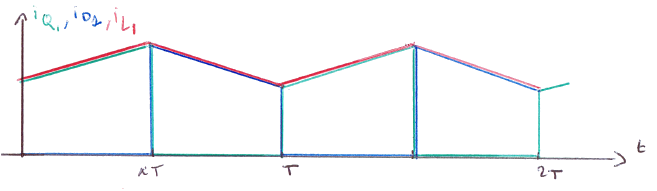
\includegraphics[width=\textwidth]{TD_Boost_2Q_Onduleur/Correction/fig/Boost_currents.PNG}
    \end{figure}

    \begin{figure}[H]
        \centering
        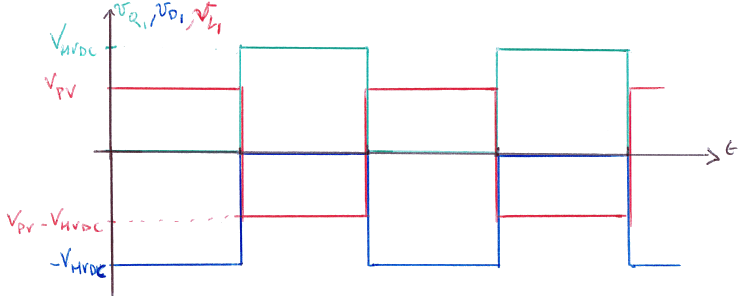
\includegraphics[width=\textwidth]{TD_Boost_2Q_Onduleur/Correction/fig/Boost_voltages.PNG}
    \end{figure}

    \item \ 
    
    $\begin{aligned}
        <v_{L1}> = 0 &\Rightarrow \alpha V_{PV} +(1-\alpha)(V_{PV} -V_{HVDC})=0\\
        &\Rightarrow V_{HVDC} = \dfrac{V_{PV}}{1-\alpha}
    \end{aligned}$

    \begin{itemize}
        \item \underline{No losses} $\Rightarrow V_{PV}\cdot I_{PV} = V_{HVDC} \cdot I_{HVDC}$
        
        $\Rightarrow I{PV}= \dfrac{I_{HVDC}}{1-\alpha}$
    \end{itemize}

    \item \  

        \begin{tabular}{|c|c|c|c|}
            \hline
            & Max Voltage & Max Current & Average Current \\
            \hline
            $L_1$ & $Max(V_{PV};|V_{PV}-V_{HVDC}|)$ & $I_{PV} + \dfrac{\Delta I}{2}$ & $I_{PV}$\\
            \hline
            $Q_1$ & $V_{HVDC}$ & $I_{PV} + \dfrac{\Delta I}{2}$ & $\alpha I_{PV}$ \\
            \hline
            $D_1$ & $V_{HVDC}$ & $I_{PV} + \dfrac{\Delta I}{2}$ & $(1-\alpha) I_{PV}$\\
            \hline
        \end{tabular}
\newpage
        \item 
        \begin{itemize}
            \item STC : 1 pannel : $250 \text{W}_C$
            $\Rightarrow \text{11 panels : } P_{TC} = 3000 \text{W}_C$
            
            \item Through each BOOST : $\dfrac{3000}{2}=1500 \text {W}$
            \item In the battery : $3000 - \underbrace{1500 - 300}_{\text{max power consumed}} = 1200 \text{ W}$
        \end{itemize}

        \item \begin{enumerate}
            \item 1 panel @ STC $\rightarrow V_{1PV} = 39 V$
            $\Rightarrow \text{6 panels in series} \rightarrow V_{PV} = 234 \text{ V}$

            \item 1 Boost $\rightarrow P = 1500 \text{ W} \Rightarrow I_{PV} = \dfrac{1500}{234} = 6.4 \text{ A}$
            \item $V_{HVDC} = 500 \text{ V} \Rightarrow \alpha = \dfrac{V_{HVDC} - V_{PV}}{V_{HVDC}} = 0.53$
            \item $I_{PV} = 6.4 \text{ A} \Rightarrow \Delta I = 1.28 \text{ A}$ (20\% if $I_{PV}$)
            \newline \underline{$0 < t < \alpha t$} : $V_L = V_{PV} = L \dfrac{i_{PV}}{dt} \Rightarrow \Delta I = \dfrac{V_{PV}}{L}\alpha T$
            \newline $\Rightarrow L = 1.93 \text{ mH}$
            \item \ 
            
            \begin{tabular}{|c|c|c|c|}
                \hline
                & Max Voltage & Max Current & Average Current \\
                \hline
                $Q_1$ & 500 V & 7 A & 3.4 A \\
                \hline
                $D_1$ & 500 V & 7.1 A & 3 A \\
                \hline
            \end{tabular}
        \end{enumerate}

        \item 
        \begin{enumerate}
            \item $V_{PV} = 6 \times 44 = 264 \text{ V}$
            \newline 
            $\begin{array}{l l}
                \left\{\begin{array}{l l}
                \text{Battery charged} &: P_{batt} = 0 \text{ W}\\
                \text{min load} &: P_{load} = 300 \text{ W}                
            \end{array}\right. \rightarrow \text{1 BOOST : } & P=150 \text{ W} \\
            & I_{PV} = \dfrac{150}{264} = 0.57 \text{ A}\end{array}$
            \item $I_{PV} < \dfrac{\Delta I}{2} \Rightarrow$ \underline{Discontinuous mode}
            \item \ 
            \begin{figure}[H]
                \centering
                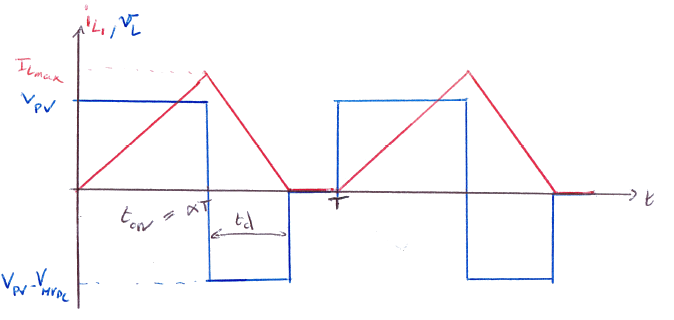
\includegraphics[width=\textwidth]{TD_Boost_2Q_Onduleur/Correction/fig/Boost_discontinuous.PNG}
            \end{figure}

            \item $<v_L> = 0 \Rightarrow V_{PV} \ cdot I_{PV} = \dfrac{I_{Lmax}}{2}\cdot \dfrac{t_{on}+t_D}{T}$
            
            \underline{$0 < t < \alpha T$} : $v_L = V_{PV} = L \dfrac{di_L}{dt} \Rightarrow I_{Lmax} = \dfrac{V_{PV}}{L} t_{on}$

            $\Rightarrow I_{PV} = \dfrac{V_{PV}}{2 L}t_{on}\cdot F_d \cdot t_{on} \left(1+\dfrac{V_{PV}}{V_{HVDC}-V_{PV}}\right)$

            $\Rightarrow I_{PV} = \dfrac{V_{PV} V_{HVDC}}{V_{HVDC}-V_{PV}}\cdot \dfrac{F_d}{2 L} \cdot t_{on}^2$
            \item $t_{on} = 8.8 \mu \text{s} \rightarrow \alpha = 0.44$
        \end{enumerate}
\end{enumerate}

% ------------------------------------- %

\newpage\section{Battery Charger}

\begin{enumerate}
    \item \ 
    \begin{figure}[H]
        \centering
        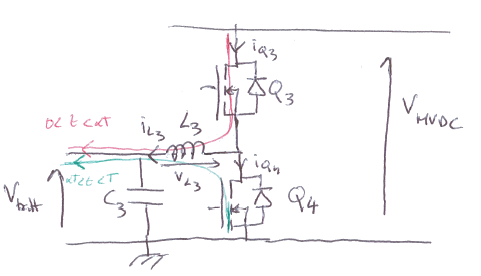
\includegraphics[width=0.9\textwidth]{TD_Boost_2Q_Onduleur/Correction/fig/HalfBridge.PNG}
    \end{figure}

    \begin{figure}[H]
        \centering
        \begin{minipage}[b]{0.45\textwidth}
            \centering \underline{Charge}
        \end{minipage}
        \hfill
        \begin{minipage}[b]{0.45\textwidth}
            \centering \underline{Discharge}
        \end{minipage}
        \vfill
        \begin{minipage}[b]{0.45\textwidth}
            \centering
            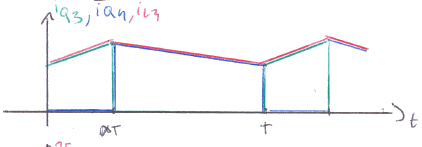
\includegraphics[width=\textwidth]{TD_Boost_2Q_Onduleur/Correction/fig/HalfBridge_current_charge.PNG}
        \end{minipage}
        \hfill
        \begin{minipage}[b]{0.45\textwidth}
            \centering
            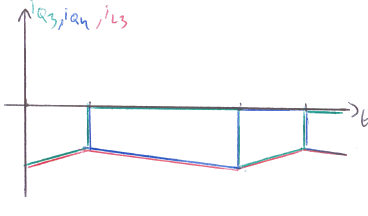
\includegraphics[width=\textwidth]{TD_Boost_2Q_Onduleur/Correction/fig/HalfBridge_current_discharge.PNG}
        \end{minipage}
        \vfill
        \begin{minipage}[b]{0.45\textwidth}
            \centering
            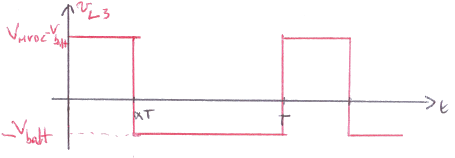
\includegraphics[width=\textwidth]{TD_Boost_2Q_Onduleur/Correction/fig/HalfBridge_voltage.PNG}
        \end{minipage}
        \hfill
        \begin{minipage}[b]{0.45\textwidth}
            \centering
            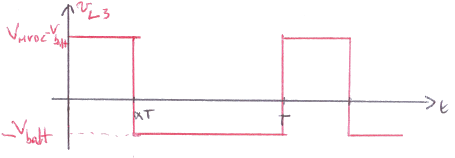
\includegraphics[width=\textwidth]{TD_Boost_2Q_Onduleur/Correction/fig/HalfBridge_voltage.PNG}
        \end{minipage}
    \end{figure}

    \item $<v_L> = 0 \Rightarrow V_{batt} = \alpha_{HB} V_{HVDC}$
    \item \begin{itemize}
        \item $P_{batt} = 1200 \text{ W} \rightarrow \text{battery charging} \rightarrow \text{Half Bridge in Buck}$
        \item $C_3$ is used to filter hight frequency current ripple so it does not flow in the Battery
    \end{itemize}

    \item \begin{enumerate}
        \item $I_{batt} = \dfrac{P_{batt}}{V_{batt}}=\dfrac{1200}{120} = 10\text{ A} \rightarrow \Delta I = 3\text{ A}$
        
        $V_{batt} = 120\text{ V}, V_{HVDC} = 500 \text{ V} \rightarrow \alpha_{HB} = 0.24$
        \item \underline{$0 < t < \alpha T$} : $V_{L}= V_{HVDC} - V_{batt} = L \dfrac{di_L}{dt}$ 
        
        $\Rightarrow \Delta I = \dfrac{V_{HVDC}-V_{batt}}{L} \alpha T \Rightarrow L = 600 \mu\text{H}$
    \end{enumerate}

    \item \ 
    
    \begin{tabular}{|c|c|c|c|}
        \hline
        & Max Voltage & Max Current & Average Current \\
        \hline
        $Q_3$ & 500 V & 11.5 A & 2.4 A ($\alpha I_{batt}$) \\
        \hline
        $Q_4$ & 500 V & 11.5 A & 7.6 A ($(1-\alpha)I_{batt}$)\\
        \hline
        \multicolumn{2}{c}{} &  \multicolumn{1}{c}{($I_{bat} + \dfrac{\Delta I}{2}$)} & \multicolumn{1}{c}{}
    \end{tabular}

    \item $\left\{\begin{array}{l}P_{load} = 1800 \text{ W}\\ P_{PV}=1000\text{ W}\end{array}\right. \rightarrow \left\{\begin{array}{l}P_{batt}=-800 \text{ W}\\
        I_{batt} = -6.7\text{ A}\end{array}\right.$

    \item Half Bridge in Boost operation $\rightarrow$ energy supplied by the Battery
    \item $\alpha_{HB}=0.24$ ($V_{HVDC}$ and $V_{bat}$ are still the same)
    
    No discontinuous mode for Half Bridge (current reversible)

    $\rightarrow$ current in $L_3$ is just negative

    \begin{center}
        \begin{minipage}[c]{0.2\textwidth}
            \centering
            \underline{$0 < t < \alpha_{HB} T$} :
        \end{minipage}
        \hfill
        \begin{minipage}[c]{0.5\textwidth}
            \centering
            
\includegraphics[width=\textwidth]{TD_Boost_2Q_Onduleur/Correction/fig/HalfBridge_1.PNG}
        \end{minipage}
        \hfill
        \begin{minipage}[c]{0.2\textwidth}
            \centering
            $V_{L_3}=V_{HVDC} - V_{batt}$
        \end{minipage}
        %\vfill
        \begin{minipage}[c]{0.2\textwidth}
            \centering
            \underline{$\alpha_{HB} T < t < T$} :
        \end{minipage}
        \hfill
        \begin{minipage}[c]{0.5\textwidth}
            \centering
            
\includegraphics[width=\textwidth]{TD_Boost_2Q_Onduleur/Correction/fig/HalfBridge_2.PNG}
        \end{minipage}
        \hfill
        \begin{minipage}[c]{0.2\textwidth}
            \centering
            $V_{L_3}=- V_{batt}$
        \end{minipage}
    \end{center}

    \begin{figure}[H]
        \centering
        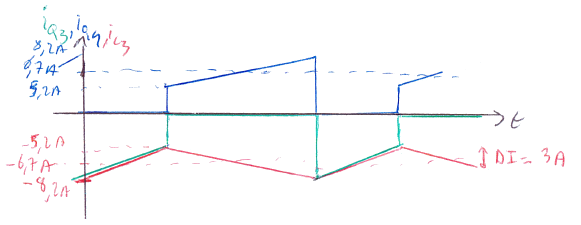
\includegraphics[width=\textwidth]{TD_Boost_2Q_Onduleur/Correction/fig/HalfBridge_current.PNG}
    \end{figure}
    
    \item \begin{enumerate}
        \item $P = 300 \text{ W} \rightarrow I_{batt} = -2.8 \text{ A}$
        \item $\alpha_{HB} = 0.24$ (Still same values of $V_{batt}$ and $V_{HVDC}$)
        
        \begin{figure}[H]
            \centering
            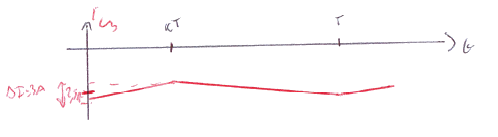
\includegraphics[width=\textwidth]{TD_Boost_2Q_Onduleur/Correction/fig/HalfBridge_currentC3.PNG}
        \end{figure}
    \end{enumerate}

    \item $P=300 \text{ W}$ \hspace{1cm} $\eta = 90\% \Rightarrow P_{batt} = 333 \text{ W}$
    
    For 16h $\rightarrow E_{batt} = 5.3 \text{ kWh}$

    Max discharge 90\% $\rightarrow E_{batt TOTAL} = \dfrac{E_{batt}}{0.9} = 5.9 \text{ kWh}$

    $V_{batt} = 120 \text{ V} \Rightarrow C_{batt} = 50 \text{ Ah}$

\end{enumerate}

% ------------------------------------- %

\newpage \section{Single-Phase PWM Inverter on RL Load}

\begin{figure}[H]
    \centering
    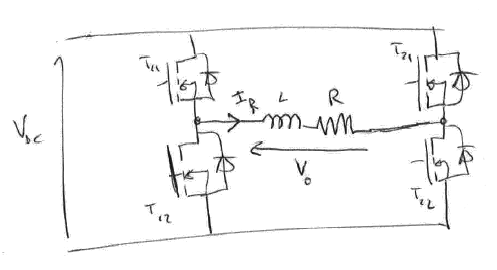
\includegraphics[width=\textwidth]{TD_Boost_2Q_Onduleur/Correction/fig/Inverter.PNG}
\end{figure}

$$\alpha(t) = 0.5 + \delta_\alpha \sin(\omega t)$$

\begin{enumerate}
    \item \begin{enumerate}
        \item \ 
        \begin{figure}[H]
            \centering
            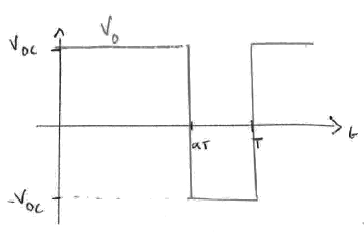
\includegraphics[width=\textwidth]{TD_Boost_2Q_Onduleur/Correction/fig/Inverter_voltage.PNG}
        \end{figure}

        \item $<V_0> = (2\alpha - 1) V_{DC}$
        \item $<V_0> (t) = (2\alpha(t) - 1 ) V_{DC} = 2\delta_\alpha V_{DC} \sin(\omega t)$
        \item $V_{0 eff} = \sqrt{2} \delta_\alpha V_{DC}$
        \item $I_{R eff} = \dfrac{V_{0 eff}}{\sqrt{R^2 + (L\omega)^2}}$
        \item $\tan \delta = \dfrac{L\omega}{R}\Rightarrow \varphi = \arctan(\dfrac{L\omega}{R})$
        \item $pf=\cos\varphi=cos(\arctan(\dfrac{L\omega}{R}))$
        \item \ 
        
        $\begin{aligned}P_R &=R \cdot I_{R eff}^2= \dfrac{R V_{0 eff}^2}{R^2 + (L\omega)^2}= \dfrac{2 R \delta_\alpha^2 V_{DC}^2}{R^2 + (L\omega)^2}\\
            &= \dfrac{2\delta_\alpha^2 V_{DC}^2}{R} \cdot \dfrac{1}{1+ \tan^2 \varphi} 
        \end{aligned}$
    \end{enumerate}
    \item \begin{enumerate}
        \item $P_R=1500 \text{ W} \hspace{1cm} U_{Rn} = 230 \text{ V} \Rightarrow I_{Rn} = \dfrac{P_R}{U_{Rn}} = 6.5 \text{ A}$
        
        $P_R = R \cdot I_{Rn}^2 \Rightarrow R = \dfrac{P_R}{I_{Rn}^2} = 35.3 \Omega$

        Or $P_R = 500 \text{ W} = \dfrac{U_{Rn}^2}{R} \Rightarrow R \dfrac{U_{Rn}^2}{P_R} = \dfrac{230^2}{1500} = 35.3 \Omega$
        \item $L=30 \text{ mH} \hspace{1cm} f=50 \text{ Hz} \Rightarrow \varphi = \arctan(\dfrac{L\omega}{R}) = 0.26 (15^\circ)$
        
        $\cos \varphi = 0.97$
        \item \ 
        \begin{figure}[H]
            \centering
            
\includegraphics[width=0.5\textwidth]{TD_Boost_2Q_Onduleur/Correction/fig/Inverter_Fresnel.PNG}
        \end{figure}
        
        \item $I_R= 6.5 \text{ A} \rightarrow V_L = L \omega I_R = 61.23 \text{ V}$
        \item $V_{0 eff} = \sqrt{U_R^2 + V_L^2} = 238 \text{ V}$
        \item $V_{0 eff} = \sqrt{2} \delta_\alpha V_{DC}$ with $V_{DC} = 500 \text{ V} \Rightarrow \delta_\alpha = \dfrac{V_{0 eff}}{\sqrt{2} V_{DC}} = 0.34$
    \end{enumerate}
    \item Max voltage : $\dfrac{V_{DC}}{2} = 250 \text{ V}$
    
    Max current : $\dfrac{V_{0 eff} \sqrt{2}}{\sqrt{R^2 + (L\omega)^2}} = \dfrac{\sqrt{2} \delta_\alpha V_{DC} \sqrt{2}}{\sqrt{R^2 + (L\omega)^2}} = 9.3 \text{ A}$
\end{enumerate}